\chapter{System Model}
\section{Use Case Models}

\subsection{UC\_QualityMetricsExtractor\_0.1}

	\begin{figure}[ht]
	\centering
	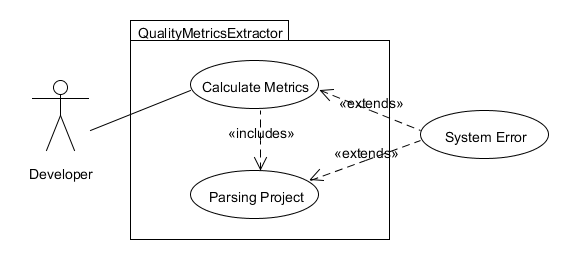
\includegraphics[scale=0.6]{img/usecase1.png}
	\caption{Use Case Diagram}\label{fig:usecase1}
	\end{figure}
		
%template caso d'uso
\begin{usecase}
\addtitle{Nome Use Case}{Calcolo metriche}
\addfield{ID:}{UC\_QualityMetricsExtractor\_0.1}
\addfield{Partecipanti:}{Sviluppatore}
\addfield{Condizioni di ingresso:}{Lo sviluppatore avvia la IDE "Eclipse"}
\addscenario{Flusso di eventi:}{
	\item Lo sviluppatore avvia il tool tramite il tasto "run".
	\item "SIE" apre una finestra della IDE mostrando sulla sinistra la lista dei progetti che è possibile analizzare.
	\item Lo sviluppatore seleziona il progetto, e da' avvio al programma.
	\item "SIE" notifica l'avvenuto calcolo delle metriche tramite un messaggio che compare in console.
}
\addfield{Condizioni di uscita:}{
	\begin{enumerate}
	\item[a.] Il sistema memorizza i dati.
	\item[b.] Lo sviluppatore termina precocemente l'operazione di calcolo.
	\end{enumerate}
}
\addfield{Eccezioni:}{Errore di sistema}
\end{usecase}

\subsection{UC\_ChangeConfigSettings}

	\begin{figure}[ht]
	\centering
	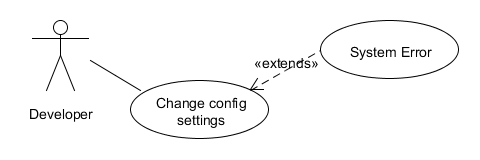
\includegraphics[scale=0.6]{img/usecase2.png}
	\caption{Use Case Diagram}\label{fig:usecase1}
	\end{figure}
	
\begin{usecase}
\addtitle{Nome Use Case}{Modifica file di configurazione}
\addfield{ID:}{UC\_ChangeConfigSettings}
\addfield{Partecipanti:}{Sviluppatore}
\addfield{Condizioni di ingresso:}{Il plugin è installato correttamente nell'IDE eclipse.}
\addscenario{Flusso di eventi:}{
	\item Lo sviluppatore apre il file settings.config con un qualsiasi editor di testo.
	\item Lo sviluppatore configura le metriche da calcolare.
}
\addfield{Condizioni di uscita:}{
	\begin{enumerate}
	\item[a.] Il plugin è configurato per le metriche desiderate.
	\item[b.] Lo sviluppatore ha scritto male i dati di configurazione.
	\end{enumerate}
}
\addfield{Eccezioni:}{Errore di sistema}
\end{usecase}

\section{Object Models}
La struttura dell'intero sistema software si sintetizza nel modello a oggetti rappresentato dal seguente diagramma.
\begin{figure}[ht]
	\centering
	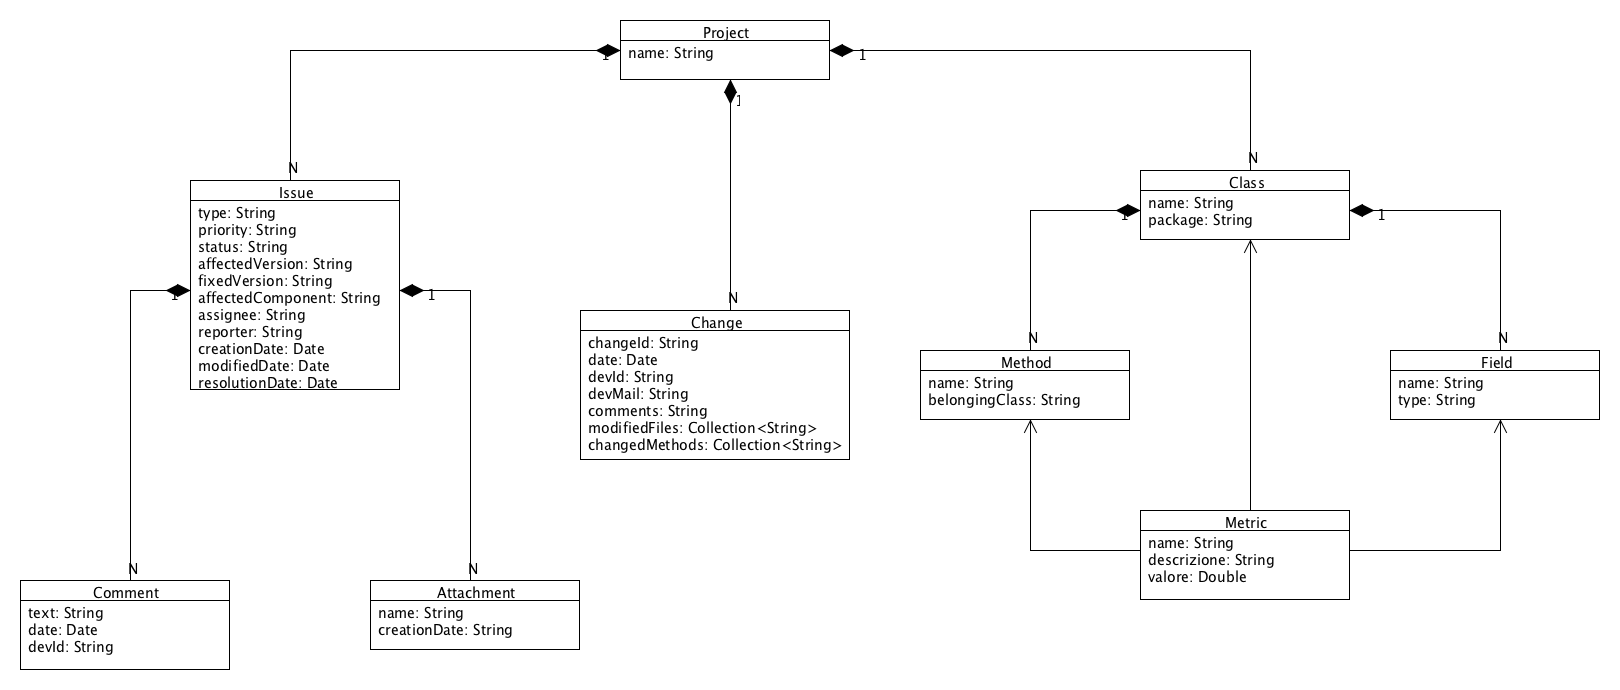
\includegraphics[scale=0.3, angle=90]{img/objectModel.png}
	\caption{Modello a oggetti}\label{fig:objectModel}
\end{figure}

